
\subsection{Experimentation}
\label{subsec:experiments2}

We highlight the improvements brought to epidemic dissemination protocols on a
real-life use case concerning decentralized collaborative editing in web
browsers.  These experiments run on Grid'5000 testbed and involve up till 600
browsers simultaneously writing a document. Using \SPRAY, we expect a traffic
logarithmically scaling compared to the network size, along with a
polylogarithmic growth brought by the real-time editor itself. 

\vspace{-7pt}
\paragraph{CRATE on network of browsers}

\begin{figure}
  \centering
  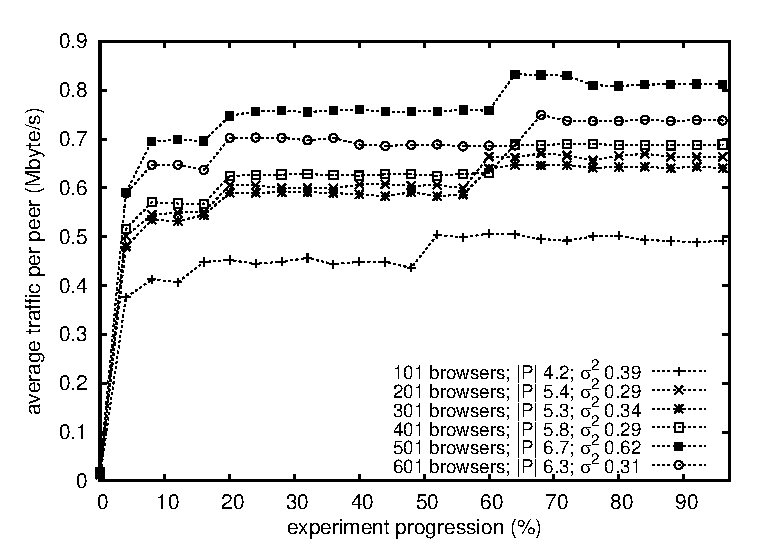
\includegraphics[width=0.49\textwidth]{img/traffic.eps}
  \caption{\label{fig:traffic}Average traffic per second.}
\end{figure}

\begin{asparadesc}
\item [Objective:] To show the influence of \SPRAY's adaptiveness over the
  traffic generated by decentralized editors running on a network of browsers.
\item [Description:] Experiments run on Grid'5000 where machines host 5 browsers
  each. Browsers open \CRATE and connect to an editing session through a
  signaling server.  Runs comprise from 101 browsers to 601 browsers with 100
  browsers increments, i.e., 6 different runs.  The first editor creates the
  editing session which is progressively joined by the other writers (1 joiner
  per 5 seconds). Each member starts sharing the access to the editing session
  as soon as it joins it. Hence, outsiders join the network through one of them
  chosen at random. Once all peers have joined the editing session, they start
  inserting characters in the document. The insertion rate is 100 insertions per
  second uniformly distributed among peers. Each experiment runs during 8 hours
  of which 7 hours are dedicated to editing. The document size reaches millions
  of characters.
\item [Results:] Figure~\ref{fig:traffic} shows the average traffic per second
  of members involved in the editing session. The x-axis denotes the time
  progression of the experiment in percentage over the 7 hours. The y-axis
  denotes the traffic generated by each browser in megabytes per second, i.e.,
  100 operations are broadcast. Legend shows the average partial view and the
  variance associated with each run. The height of the plots corresponds to the
  multiplicative factor coming from the messages dissemination. As expected,
  this factor grows logarithmically regarding the network size. Thus, 101
  browsers have an average traffic lower than 601 browsers because their partial
  views are smaller in average.  On the opposite, using \CYCLON, the traffic
  would have been the same for all runs. Since it commonly overestimates partial
  views to accommodate with any network size, the traffic would have been higher
  (cf. Figure~\ref{fig:churn}). It is important since we observe that even small
  partial view size differences significatively impact traffic.
  Figure~\ref{fig:traffic} also shows that the average partial view size follows
  the natural logarithmic expectation. Yet, the run involving 501 browsers has a
  slightly higher average partial view size than the run involving 601
  browsers. Because the joining part of \SPRAY establishes a number of WebRTC
  connections depending on the first contact member, there are variations
  between independant runs. Still, \SPRAY scales logarithmically
  overall. Figure~\ref{fig:traffic} finally shows that the variance remains
  small which indicates that the network of browsers reached a state where
  neighborhood size are balanced, hence, where the load is balanced.
\item [Reasons:] Broadcast uses neighborhoods to disseminate messages. Each
  member receives and forwards each operation which transitively reaches all
  members. Thus, the traffic depends of messages size multiplied by
  neighborhoods size logarithmically scaling thanks to \SPRAY. The growth during
  each run corresponds to the polylogarithmic growth of identifiers from the
  editors. The document size increases over time, the depth of the \LSEQ tree
  representing the document increases accordingly. Nevertheless, since the
  maximum arity of the tree increases over levels, the more the document grows
  the less the tree grows.
\end{asparadesc}
